\documentclass[11pt]{article}
\usepackage[T1]{fontenc}
\usepackage[utf8]{inputenc}
\usepackage{lmodern,amsmath,amssymb,graphicx,geometry,microtype,setspace,booktabs,caption}
\usepackage[hidelinks]{hyperref}
\geometry{letterpaper,margin=1in}
\setlength{\parindent}{0pt}
\setlength{\parskip}{0.55em}
\setlength{\emergencystretch}{2em}
\captionsetup{labelfont=bf,font=small}
\renewcommand{\refname}{References}

\pagestyle{empty}
\renewcommand{\thefigure}{S\arabic{figure}}
\setcounter{figure}{6}

\begin{document}
\begin{figure}[!ht]\centering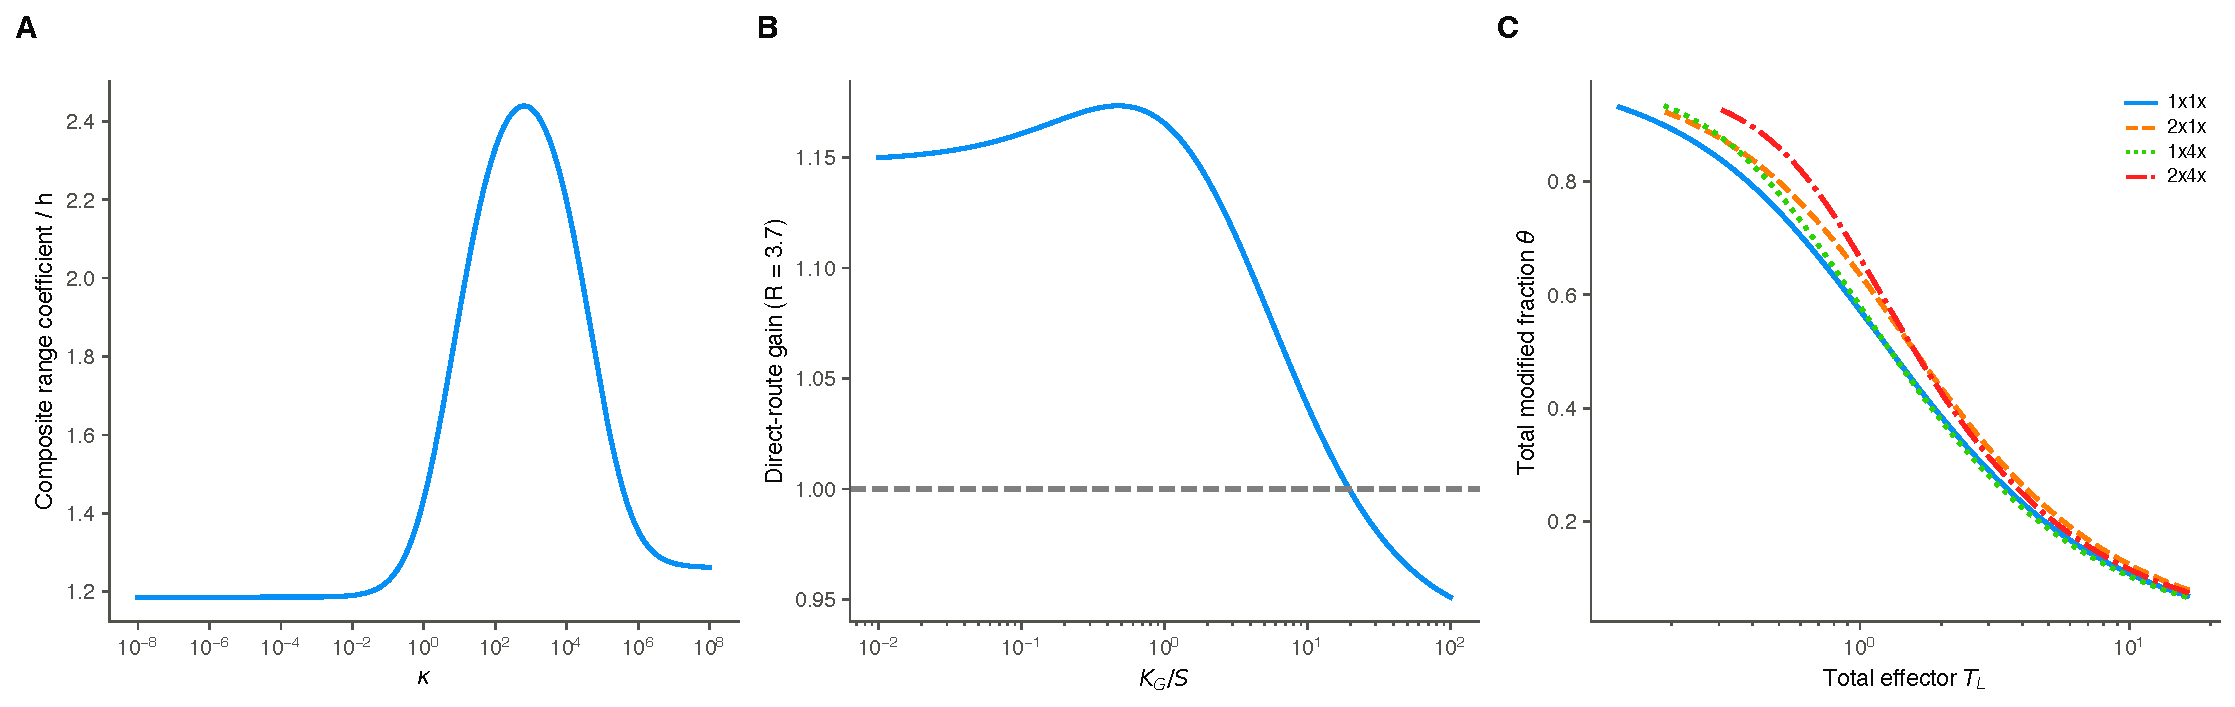
\includegraphics[width=\textwidth,height=0.65\textheight,keepaspectratio]{figure_inputs/FigS7_alternatives.pdf}\begin{singlespace}\caption{Additional consequences and competing contributions. (A) Composite response-range coefficient divided by the fitted upstream exponent as the downstream scale varies, using the linear reverse input. (B) Gain from the specified direct-activation law with R=3.7 while retaining the downstream scale calibrated before adding that law; the gain ranges approximately 0.95--1.17. (C) The high-enzyme total-effector titration from the original experimental-design figure, with baseline $T_E=0.6$, $T_S=1$ and the same independent-site constants as S8 Fig B. Legend factors vary enzyme and target independently. Curves are model predictions, not experimental traces.}\end{singlespace}\end{figure}
\end{document}
